\documentclass[a4paper,12pt]{article}
\usepackage[utf8x]{inputenc}
\usepackage{amssymb}
\usepackage{amsfonts}
\usepackage{mathrsfs}
\usepackage{amsmath}
\usepackage{amsthm}
\usepackage[margin=3cm]{geometry}
\usepackage{times}
\usepackage{graphicx}
\usepackage{enumitem}
\usepackage{fancyhdr}
\usepackage{hyperref}
\usepackage{setspace}
\usepackage{subcaption}
\usepackage{mathtools}

\pagestyle{fancy}
\fancyhf{}
\lhead{Thomas Delaney}
\rhead{COSYNE 2018 Abstract}
\cfoot{\thepage}

\newtheorem{theorem}{Theorem}
\newtheorem{proposition}{Proposition}[section]
\newtheorem{lemma}{Lemma}[section]
\newtheorem{corollary}{Corollary}[section]
\theoremstyle{definition}
\newtheorem{definition}{Definition}[section]

\newcommand{\boldnabla}{\mbox{\boldmath$\nabla$}} % to be used in mathmode
\newcommand{\cbar}{\overline{\mathbb{C}}}% to be used in mathmode
\newcommand{\diff}[2]{\frac{d #1}{d #2}}% to be used in mathmode
\newcommand{\difff}[2]{\frac{d^2 #1}{d #2^2}}% to be used in mathmode
\newcommand{\pdiff}[2]{\frac{\partial #1}{\partial #2}} % to be used in mathmode
\newcommand{\pdifff}[2]{\frac{\partial^2 #1}{\partial #2^2}}% to be used in mathmode
\newcommand{\upperth}{$^{\mbox{\footnotesize{th}}}$}%to be used in text mode
\newcommand{\vect}[1]{\mathbf{#1}}% to be used in mathmode
\newcommand{\curl}[1]{\boldnabla \times \vect{#1}} % to be used in mathmode
\newcommand{\divr}[1]{\boldnabla \cdot \vect{#1}} %to be used in mathmode
\newcommand{\modu}[1]{\left| #1 \right|} %to be used in mathmode
\newcommand{\brak}[1]{\left( #1 \right)} % to be used in mathmode
\newcommand{\comm}[2]{\left[ #1 , #2 \right]} %to be used in mathmode
\newcommand{\dop}{\vect{d}} %to be used in mathmode
\newcommand{\cov}{\text{cov}} %to be used in mathmode
\newcommand{\var}{\text{var}} %to be used in mathmode
\newcommand{\mb}{\mathbf} %to be used in mathmode
\newcommand{\bs}{\boldsymbol} %to be used in mathmode
% Title Page
\title{How informative are retinal ganglion cells?}
\author{Thomas Delaney 1330432}

\begin{document}

\subsubsection*{Title}
How do calcium indicator properties affect spike inference?

\subsubsection*{Authors}
Thomas J. Delaney, Michael C. Ashby, Cian O'Donnell

\subsubsection*{300-word Summary}
The use of fluorescent calcium indicators, such as GCaMP, to monitor neuronal activity is widespread. But the relationship between action potential firing and the fluorescence signal is poorly understood. For example, it is known that genetically encoded indicators accumulate within neurons over weeks and months. This makes comparison of activity levels at different time points difficult. Furthermore, the effects of the indicator characteristics on this fluorescence signal are unknown. As a result, it remains unknown if spike train inference is always possible using fluorescent calcium indicators.

The aim of this project was to model the fluorescence traces produced by a fluorescent calcium indicator in a neuron soma, given parameters such as binding rate, dissociation rate, and molecular concentration from a specific spike train. The ultimate goal of the model is to allow benchmarking of the various spike inference algorithms that have been developed, and to understand how indicator characteristics affect the quality of spike train inference.

The fluorescence traces produced by the model were calibrated to reproduce the signal-to-noise ratio observed in experimental data. We tested three leading spike inference algorithms (Pnevmatikakis et al. 2016, Jewell et al. 2010, Friedrich et al. 2017) on the real versus modelled calcium imaging traces. We varied the values of model parameters to determine the effect on system dynamics and on spike inference. This framework has two uses, firstly for helping experimentalists optimise their calcium imaging experiment design choices for best spike inference, and also for helping computational researchers optimise and understand their spike inference algorithms.

% We have found that low frequency fluctuations in observed fluorescence traces have a significant effect on spike inference. See figure \ref{subfig:three_algo_comparison_tp} to see spike inference quality much higher on modelled traces.

\subsubsection*{Additional Detail}
We modelled the concentrations of free calcium, fluorescent indicator, and mobile and immobile endogenous calcium buffers within the cell (see figure \ref{subfig:camodel}). The reactions between the free calcium, $[Ca^{2+}]$, and the endogenous buffers, $[X]$, are described by the following diagram:
\begin{equation*}
   [X][Ca^{2+}] \xrightleftharpoons[k_b]{k_f} [XCa]
\end{equation*}
The indicator molecules, $[B]$, bound to a calcium molecule could be either excited, i.e. able to release a photon, or relaxed. The excited molecule becomes relaxed after releasing a photon.
\begin{equation*}
   [B][Ca^{2+}] \xrightleftharpoons[k_{b}]{k_{f}} [BCa] \leftrightsquigarrow [BCa^{*}]
\end{equation*}
In order to reproduce the noise in the system dynamics, we modelled the photon release as a stochastic process.

We fitted the free parameters of the model using the Nelder-Mead algorithm, with the squared difference between the power spectrum of the real and modelled traces as the objective function.

There are existing methods for converting the fluorescence traces into spike trains. The ones we have used in this research are the constrained non-negative deconvolution algorithm (Pnevmatikakis et al. 2016), the $\ell_0$ optimisation algorithm (Jewell et al. 2010), and the online active set method to infer spikes, or OASIS algorthim (Friedrich et al. 2017). Our aim in making this model was not to infer spikes from fluoresce traces, but to model the fluorescence traces created by spike trains. See figure \ref{subfig:example_trace} for an example modelled trace, with the spike train that induced it.

Our idea is that neuroscientists designing experiments will be able to use this model to test which indicator will best suit their experimental setup. This is because they will be able to calibrate the model to imitate different fluorescent calcium indicators. Using this model, we can also test if the noisiness of the photon collection may be enough to obfuscate the spiking signal. We can also demonstrate the effects of changes in indicator characteristics on fluorescence traces, and therefore on spike inference quality. See figure \ref{subfig:indicator_perturbed_paninski_true_positive} for spike inference quality over different values of indicator concentration.

\begin{figure}[t]
  \centering
  \begin{subfigure}[b]{0.45\textwidth}
    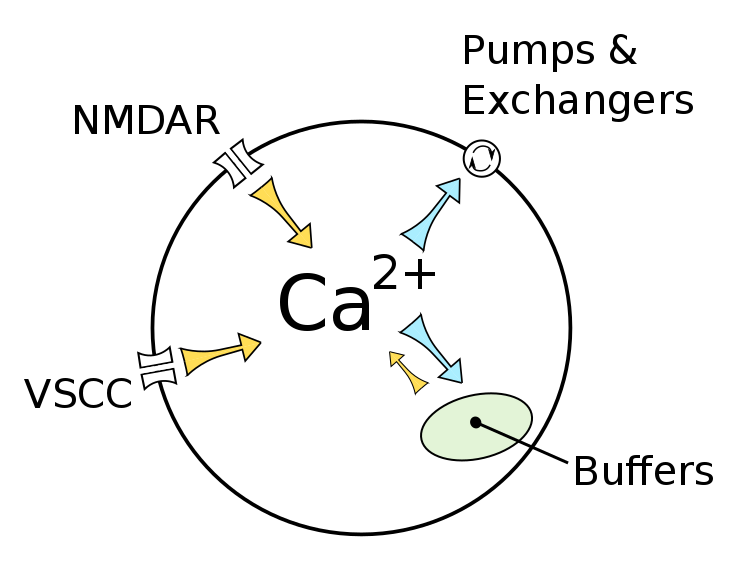
\includegraphics[width=\textwidth]{camodel.png}
    \caption{}
    \label{subfig:camodel}
  \end{subfigure}
  \begin{subfigure}[b]{0.45\textwidth}
    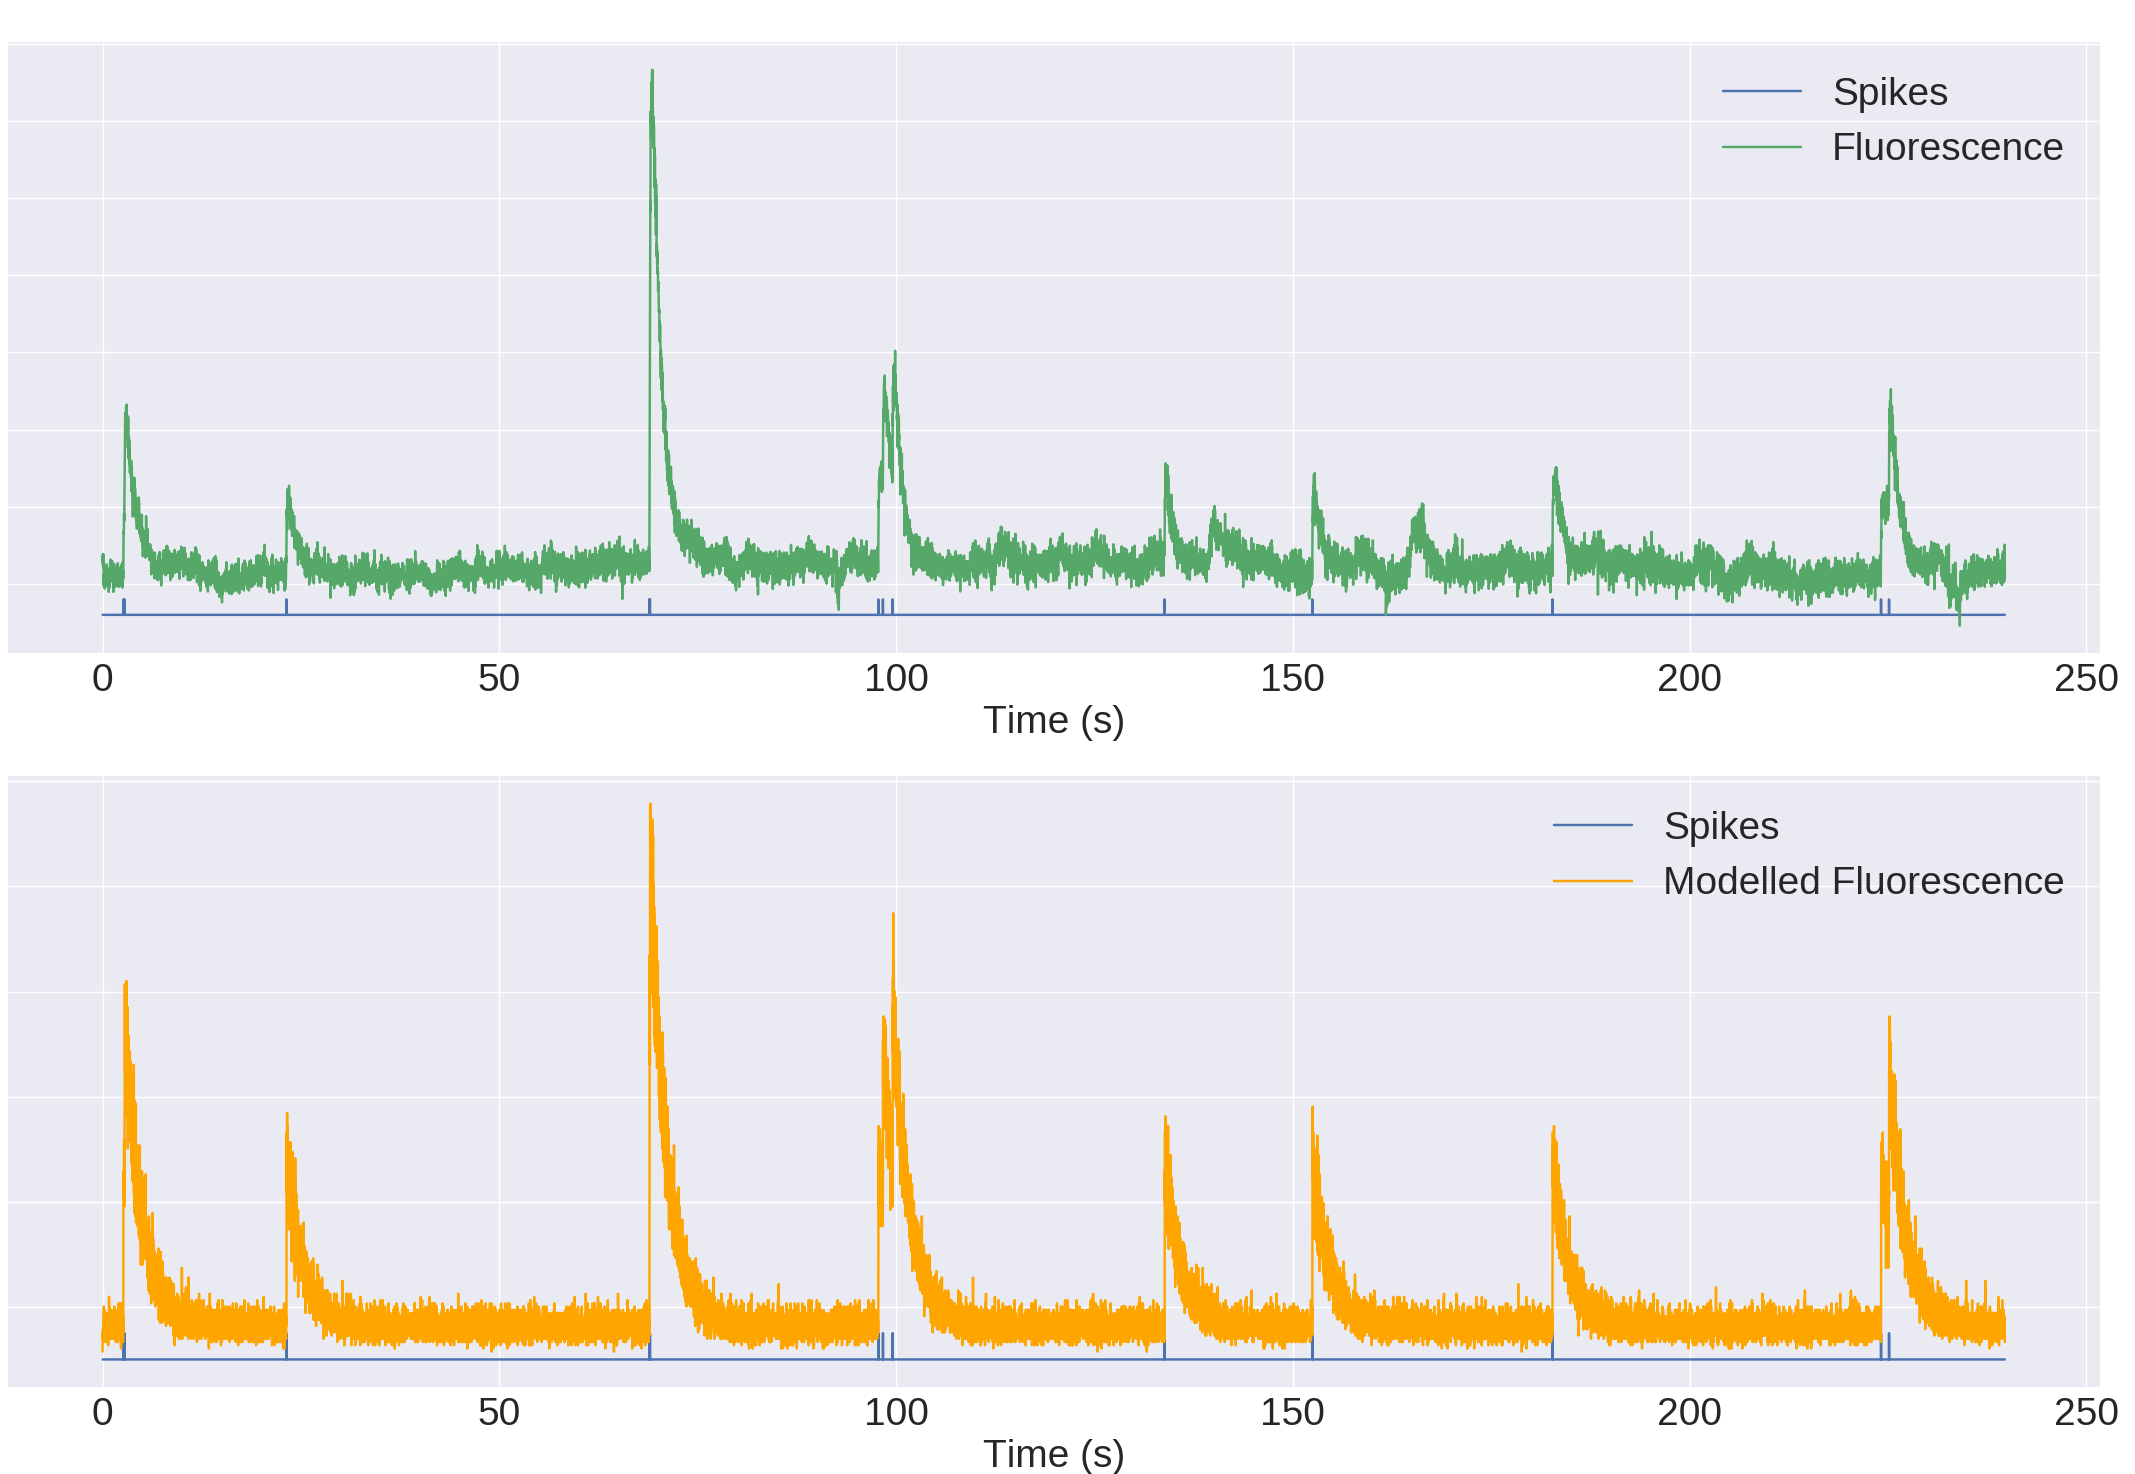
\includegraphics[width=\textwidth]{example_trace.png}
    \caption{}
    \label{subfig:example_trace}
  \end{subfigure}
  \begin{subfigure}[b]{0.45\textwidth}
    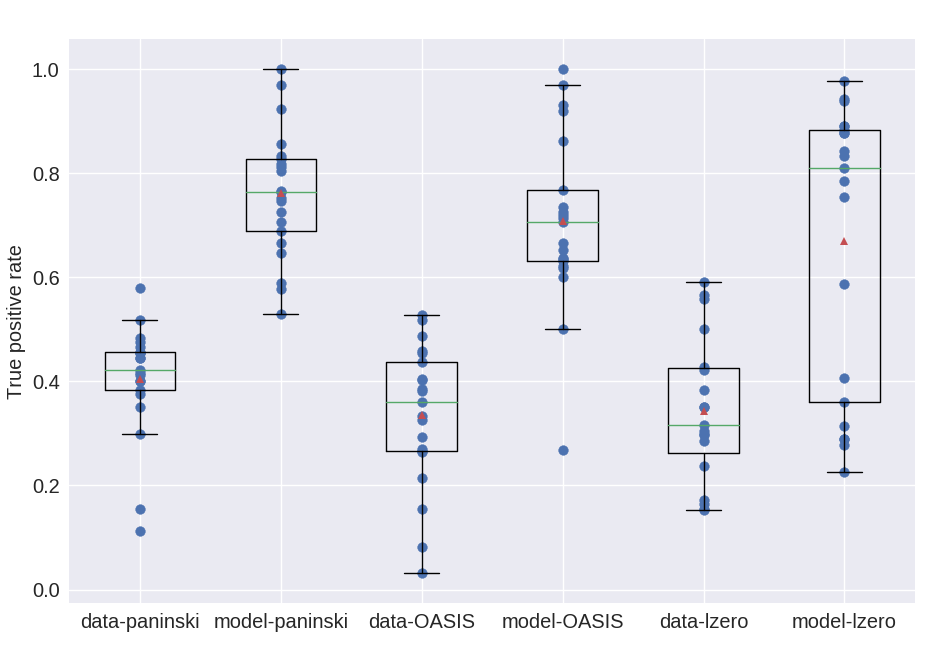
\includegraphics[width=\textwidth]{three_algo_comparison_tp.png}
    \caption{}
    \label{subfig:three_algo_comparison_tp}
  \end{subfigure}
  \begin{subfigure}[b]{0.45\textwidth}
    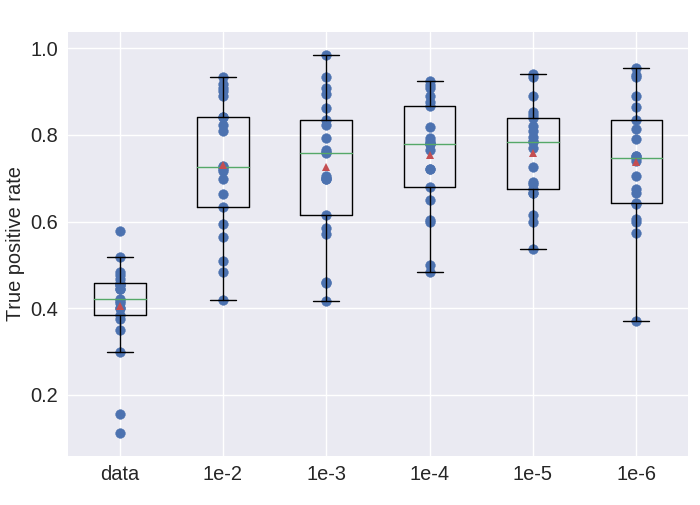
\includegraphics[width=\textwidth]{indicator_perturbed_paninski_true_positive.png}
    \caption{}
    \label{subfig:indicator_perturbed_paninski_true_positive}
  \end{subfigure}
  \caption{(a) Schematic diagram of cell calcium dynamics. (b) An example fluorescence trace with the associated modelled trace and spike train. (c) Inference quality for observed fluorescence traces and modelled fluorescence traces, measured by true positive rate. (d) Inference quality for modelled traces with perturbed values for indicator concentration.}
  \label{fig:crowded_figure}
\end{figure}

\end{document}
